% Chapter Template

\chapter{Implementación: Despliegue} % Main chapter title

\label{Chapter4} % Change X to a consecutive number; for referencing this chapter elsewhere, use \ref{ChapterX}

%----------------------------------------------------------------------------------------
%	SECTION 1
%----------------------------------------------------------------------------------------

\section{Creación máquina base}
Para poder desplegar las máquinas como servicio en los nodos de trabajo con Windows, primero se crea una máquina virtual para usarla como base.

El gestor de maquinas virtuales utilizado es \textbf{VirtualBox v 5.0.18} que se puede encontrar en la \href{https://www.virtualbox.org/wiki/Downloads}{página principal} o el enlace en la wiki de la universidad \autocite{hpc}.

\subsection*{Sistema Operativo Base}
Como sistema operativo base para el nodo de trabajo, se instala \textbf{Ubuntu 14.04} en su versión de escritorio mínima, el disco de instalación no pesa mas de 50 megas y permite instalar solo los componentes necesarios para la ejecución de y trabajos en segundo plano con la herramienta HTCondor.

Una vez instalado el gestor de máquinas virtuales, se ejecuta y se crea una nueva máquina virtual.
\begin{figure}[h]
\centering
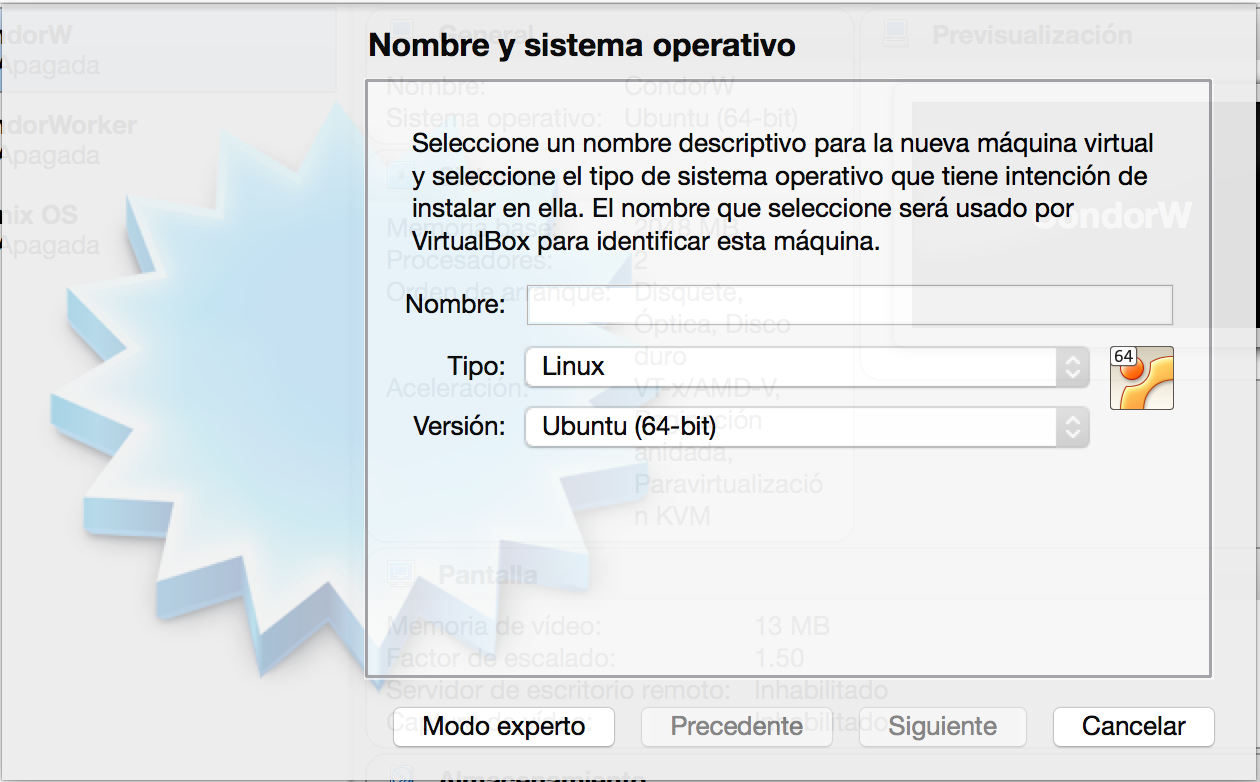
\includegraphics[width=0.7\textwidth]{vbox/newmachine.png}
\decoRule
\caption{Creación máquina virtual}
\label{fig:Nueva máquina}
\end{figure}
\FloatBarrier
Luego de seleccionar un nombre para la máquina y escoger el tipo de sistema operativo y la versión, se selecciona la memoria RAM para la máquina virtual.
\begin{figure}[h]
\centering
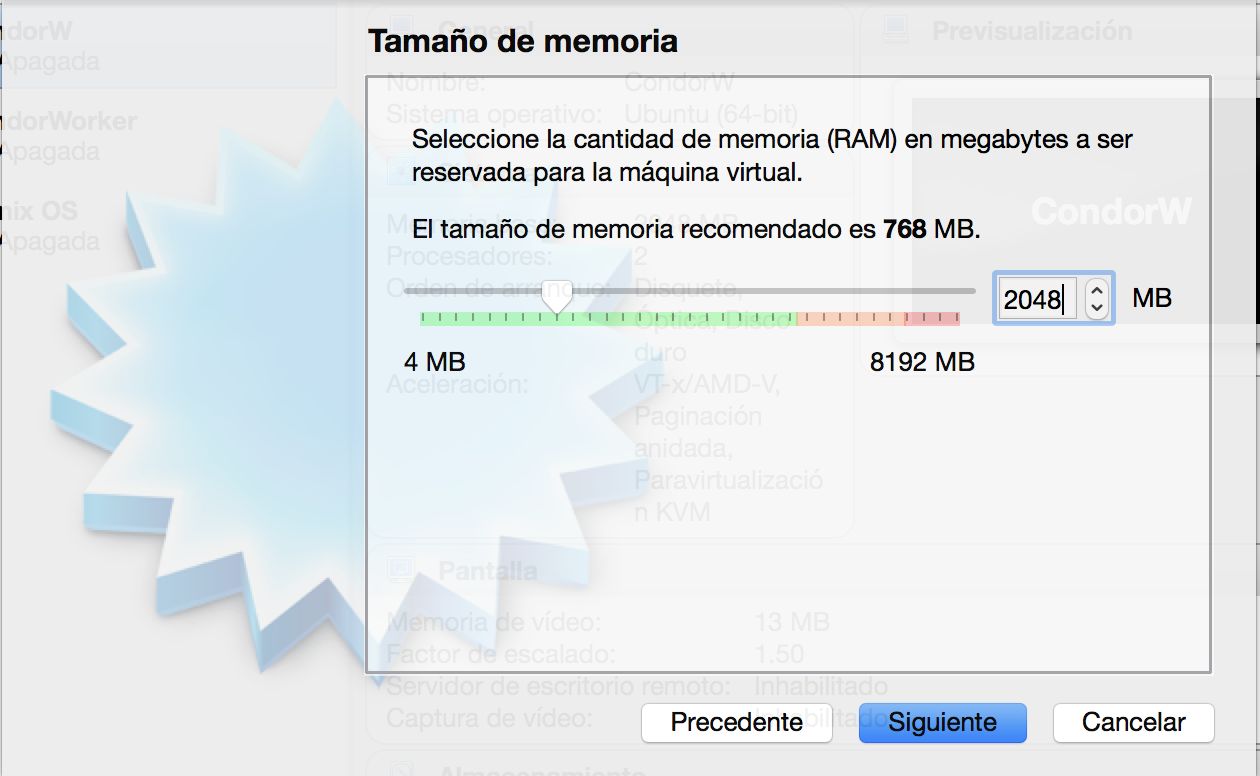
\includegraphics[width=0.7\textwidth]{vbox/memory.png}
\decoRule
\caption{Memoria máquina virtual}
\label{fig:Memoria virtual}
\end{figure}
\FloatBarrier

Se crea un disco virtual que contendrá toda la información de nuestro nodo de trabajo.
\begin{figure}[h]
\centering
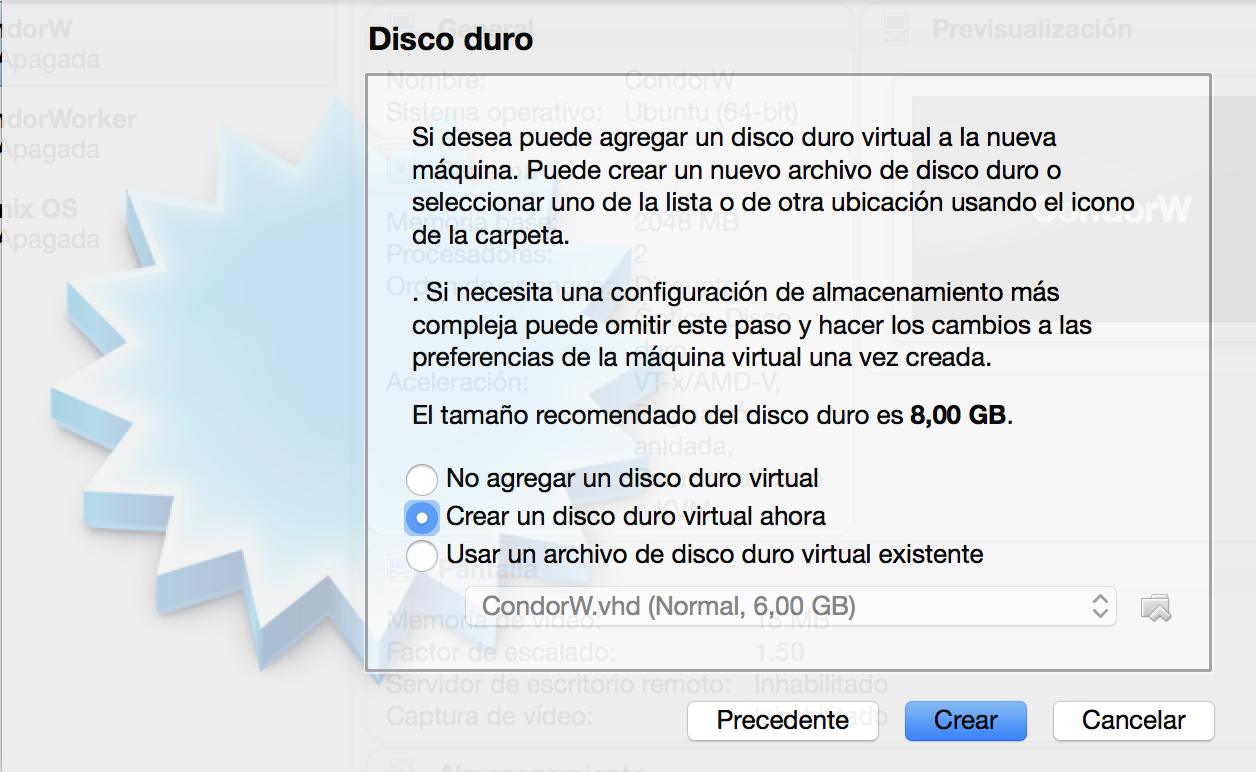
\includegraphics[width=0.7\textwidth]{vbox/virtualdisck.png}
\decoRule
\caption{Creación disco virtual}
\label{fig:Disco virtual}
\end{figure}
\FloatBarrier
El tipo de disco que se crea, en este caso es un Virtual Hard Disck (VHD) con capacidad de 10 GB.

Este espacio sera asignado de manera dinámica, así el tamaño total de la imagen del nodo de trabajo sera mas pequeña y fácil de compartir por la red de la universidad.
\begin{figure}[h]
\centering
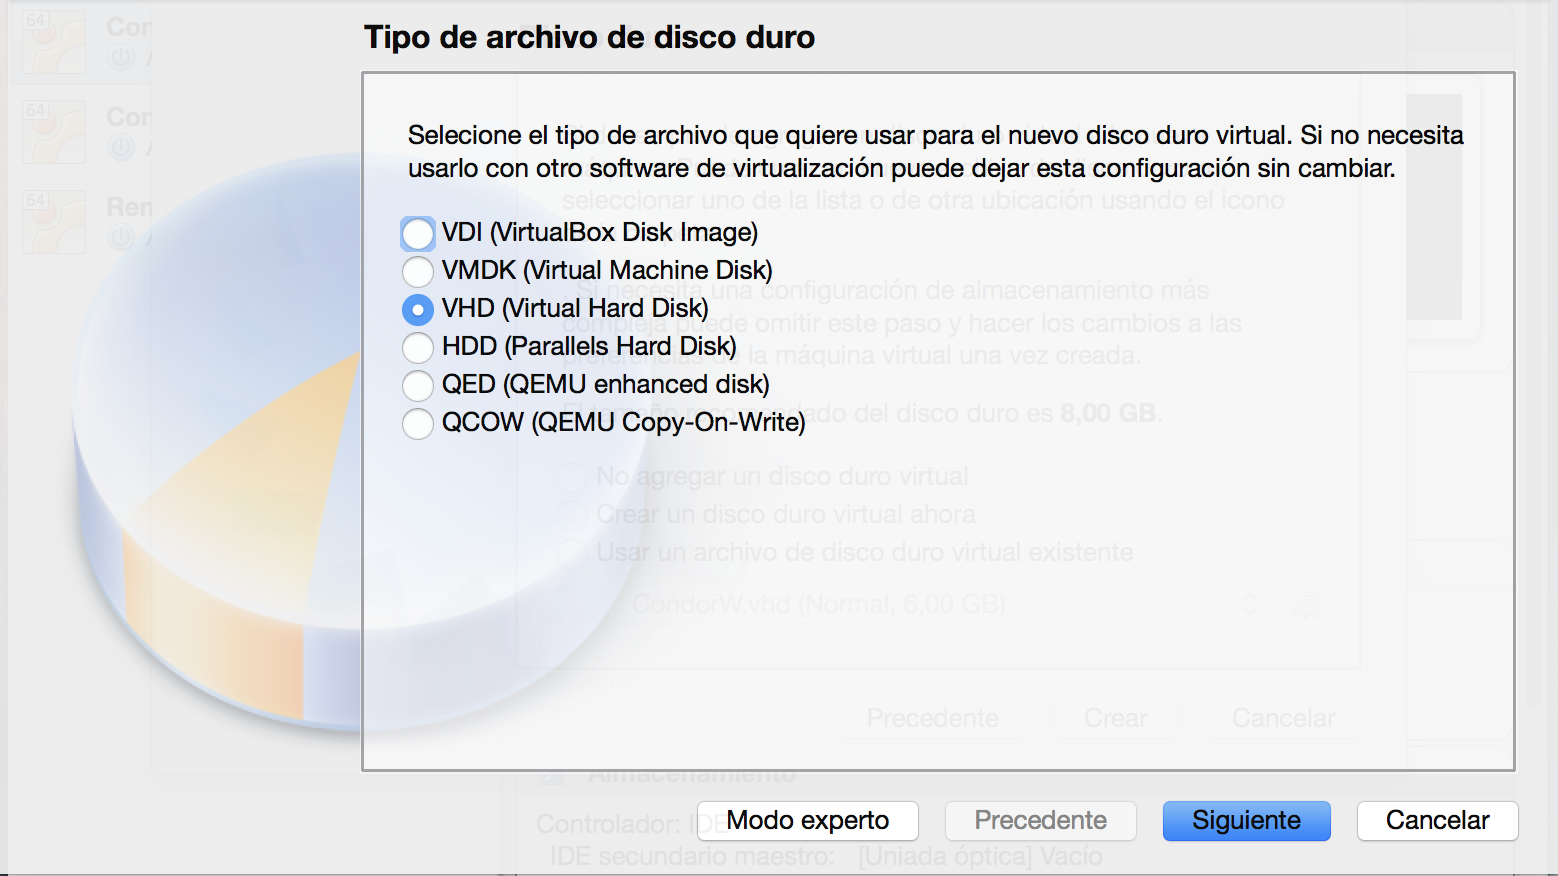
\includegraphics[width=0.7\textwidth]{vbox/vdtype.png}
\decoRule
\caption{Tipo de disco virtual}
\label{fig:hd type}
\end{figure}
\FloatBarrier

El nombre del disco virtual, es por defecto igual al nombre de la máquina virtual.

\begin{figure}[h]
\centering
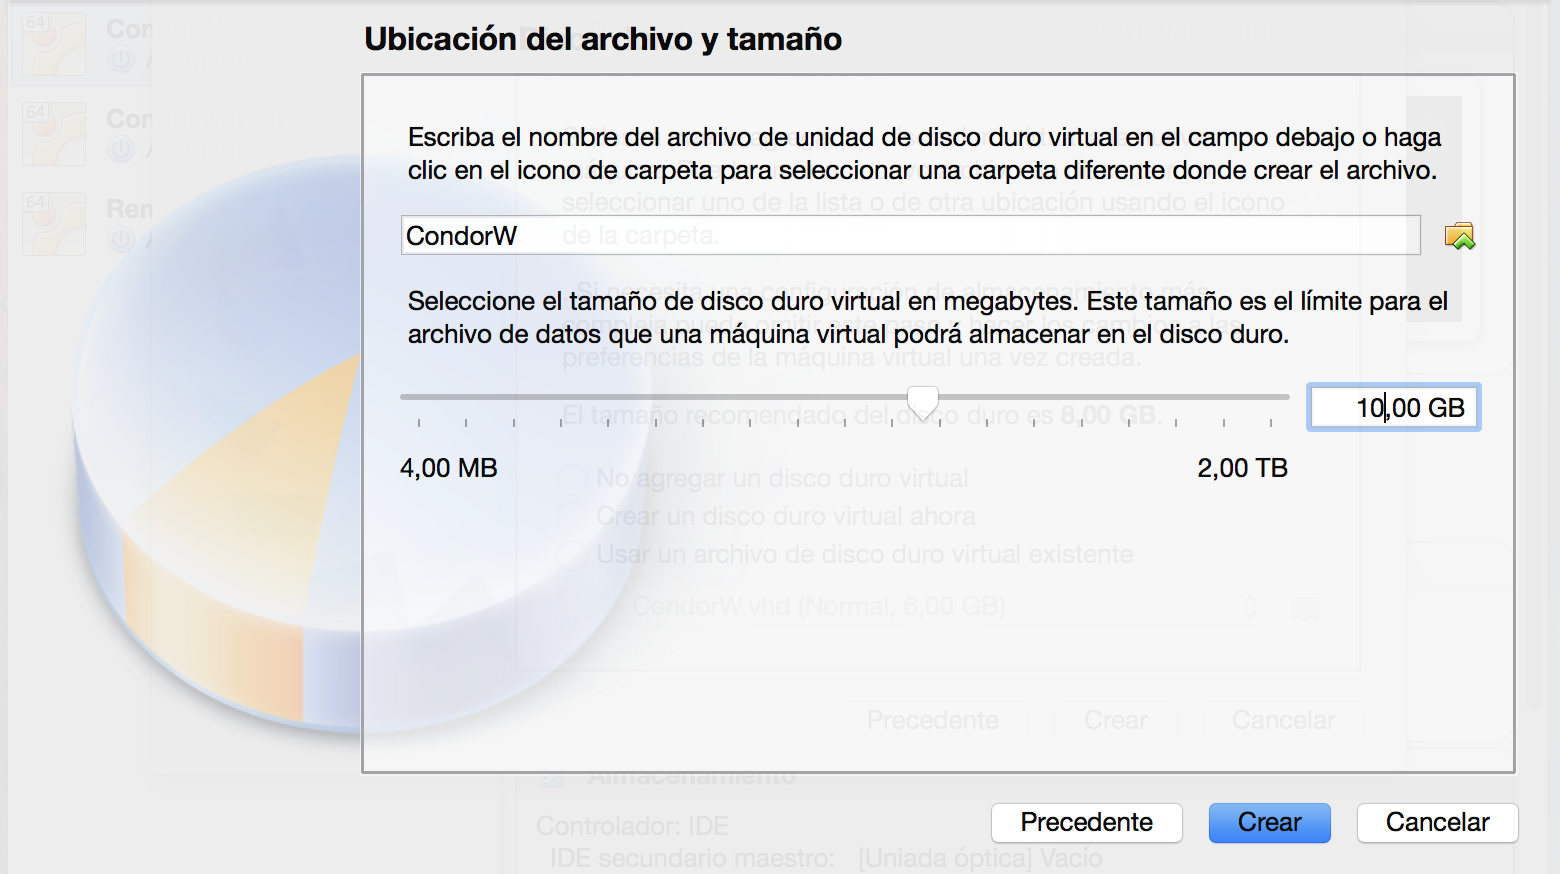
\includegraphics[width=0.7\textwidth]{vbox/vhdsize.png}
\decoRule
\caption{Tamaño disco virtual}
\label{fig:hd size}
\end{figure}
\FloatBarrier
Se le da un tamaño de 10Gb al disco virtual, por lo que se espera trabajar con grandes volúmenes de datos, pero como este disco esta asignado de manera dinámica, el tamaño final es menor al 10Gb, próximo a 3Gb.
\begin{figure}[h]
\centering
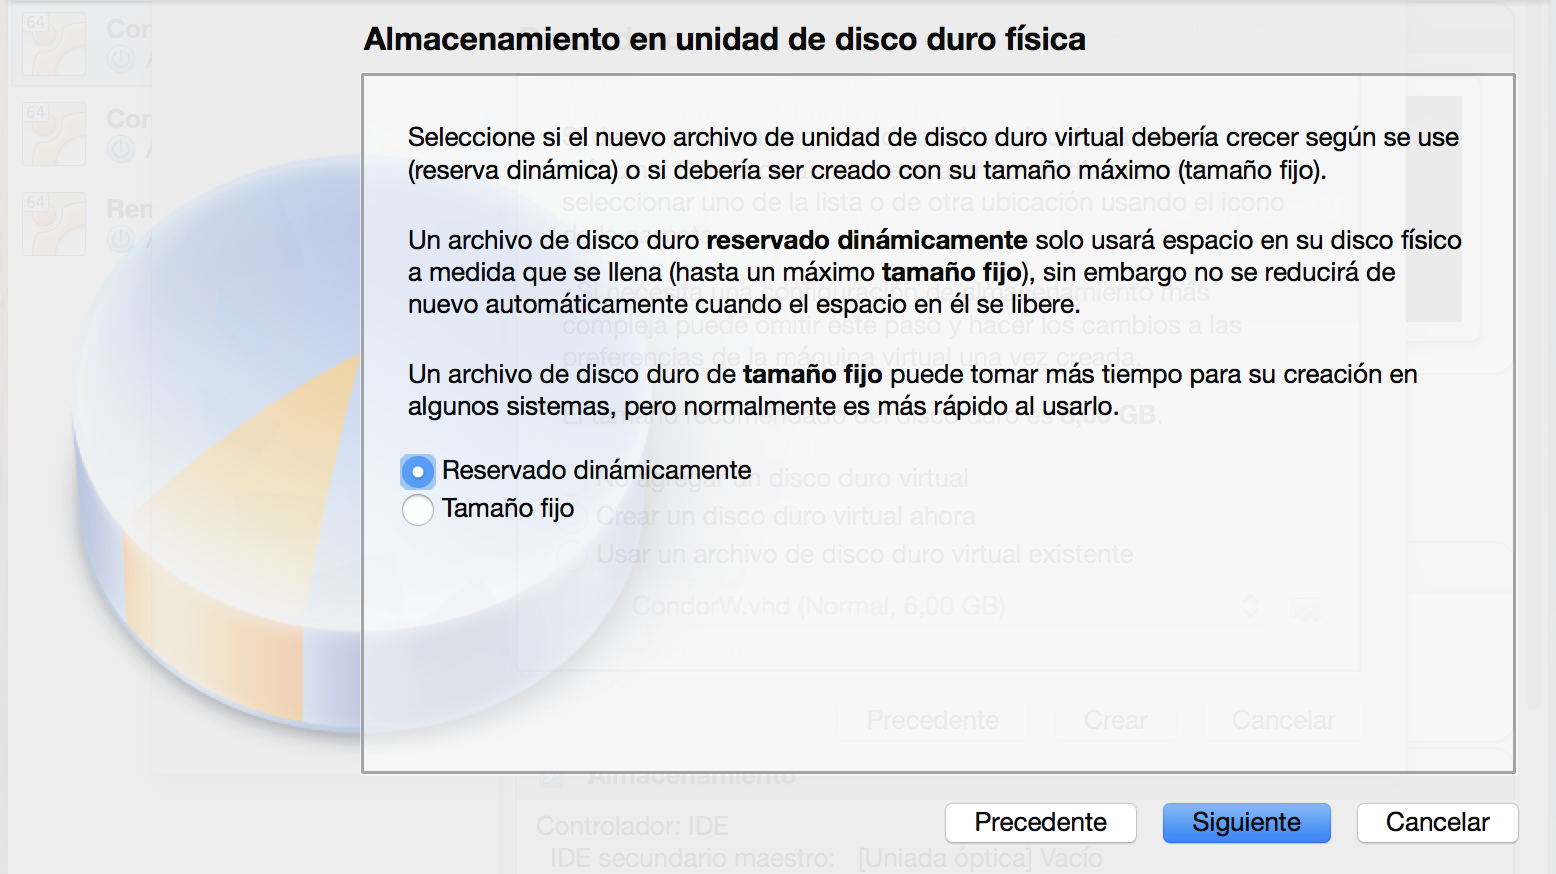
\includegraphics[width=0.7\textwidth]{vbox/dynamicvhd.png}
\decoRule
\caption{Tamaño asignado dinámico}
\label{fig:dynamic size}
\end{figure}
\FloatBarrier

Una vez creado el disco, se procede a montar la imagen del sistema operativo en una unidad virtual para la instalación en nuestra maquina.

Se realiza la instalación de Ubuntu 14.04 Desktop Minimal.

Una vez instalado el sistema operativo, accedemos a la máquina y procedemos a actualizar e instalar los paquetes necesarios para el correcto funcionamiento de HTCondor, El universo de Java, y los scripts necesario para automatizar el nombre de la máquina en el cluster.


\section{Instalación de HTCondor}
El proceso de instalación de HTCondor es realmente sencillo, se hace uso de los repositorios propios de Ubuntu para esto, una vez actualizado el sistema.

\subsection{Paso a paso}
Primero acedemos como usuario \textbf{root} e instalamos HTCondor usando el comando:

\textbf{\textit{apt-get install htcondor}}

Nos mostrará una lista de dependencias que se deben instalar para el correcto funcionamiento de la herramienta.

\begin{figure}[h]
\centering
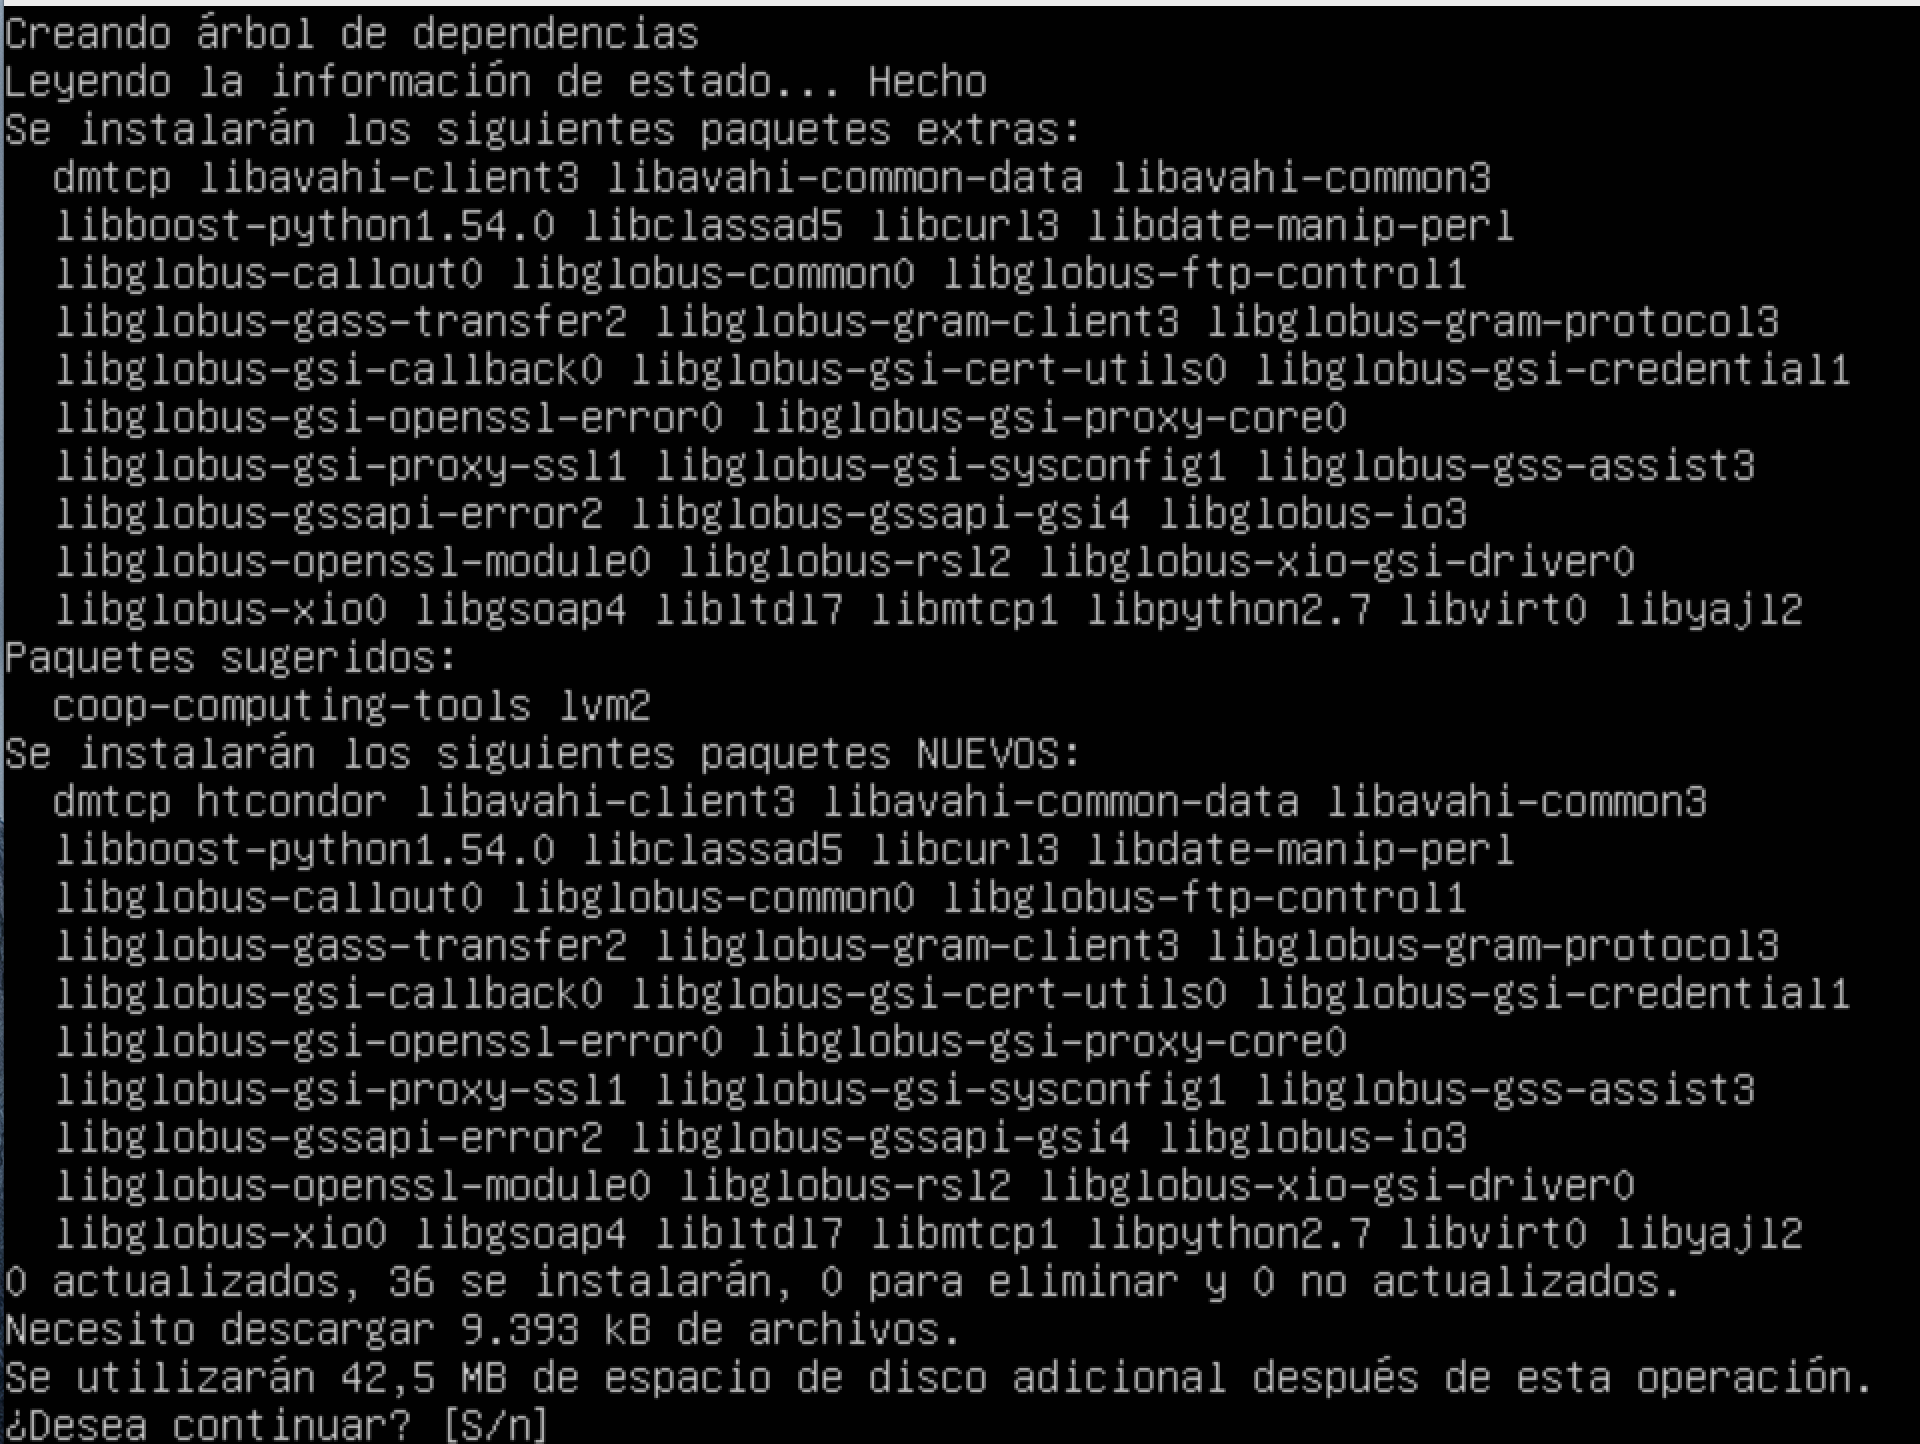
\includegraphics[width=0.8\textwidth]{Figures/dependency.png}
\decoRule
\caption{Dependencias necesarias para HTCondor}
\label{fig:htcondor dependency}
\end{figure}
\FloatBarrier

Luego nos pedirá si deseamos modificar los parámetros de configuración inicial de condor, le decimos que no, ya que el archivo de configuración lo editaremos mas adelante.

\begin{figure}[h]
\centering
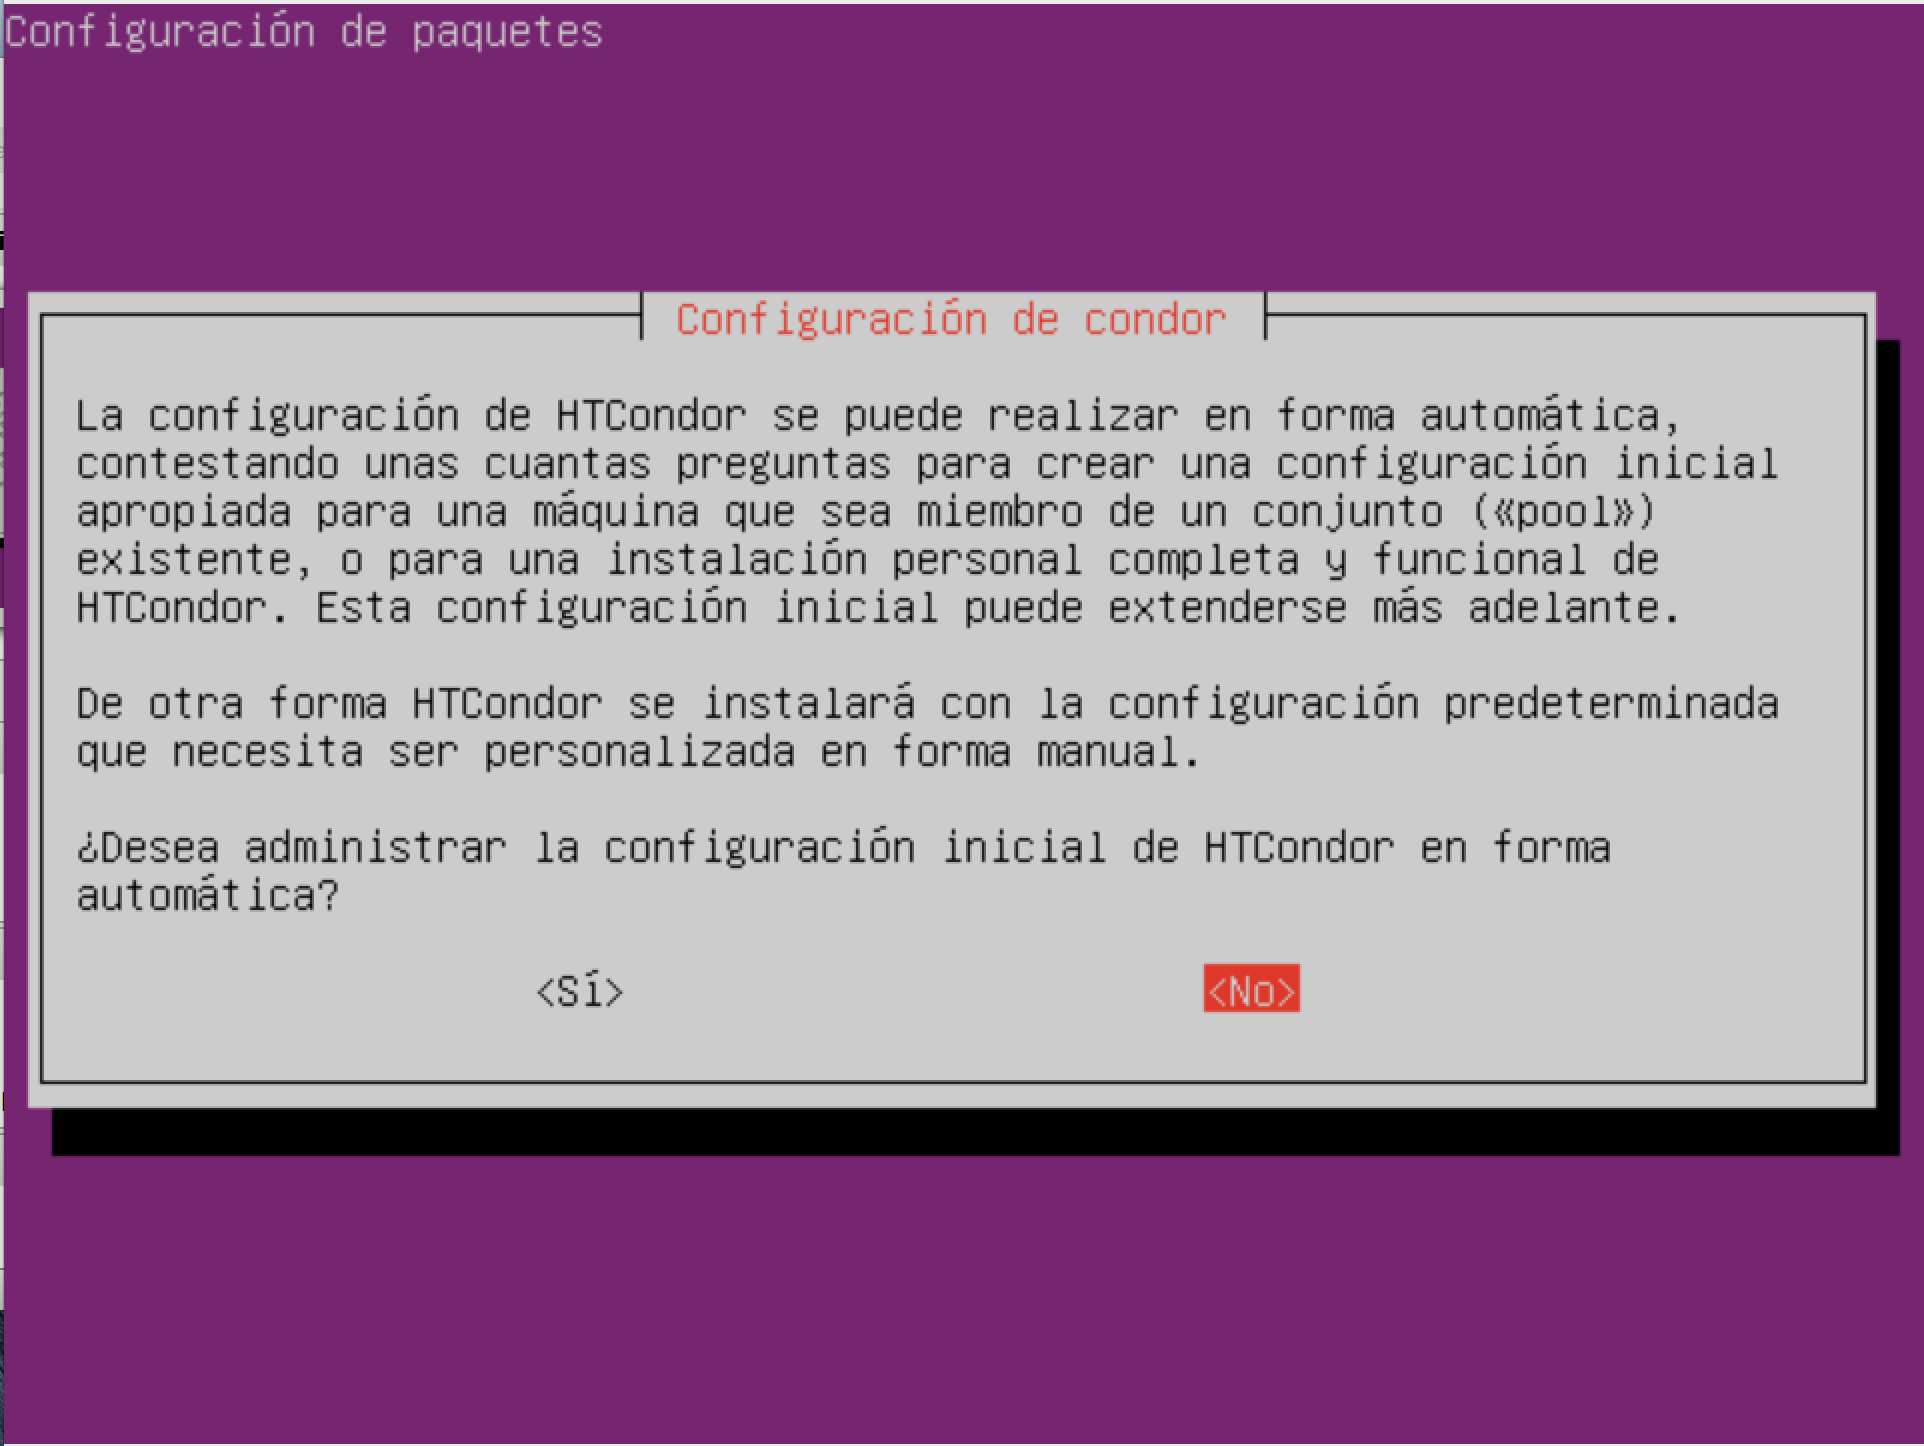
\includegraphics[width=0.8\textwidth]{Figures/preconf.png}
\decoRule
\caption{Configuración inicial}
\label{fig:htcondor pre-conf}
\end{figure}
\FloatBarrier

Verificamos que HTcondor esta correctamente instalado y ejecutándose usando el comando:

\textbf{\textit{ps aux | grep condor}}

\begin{figure}[h]
\centering
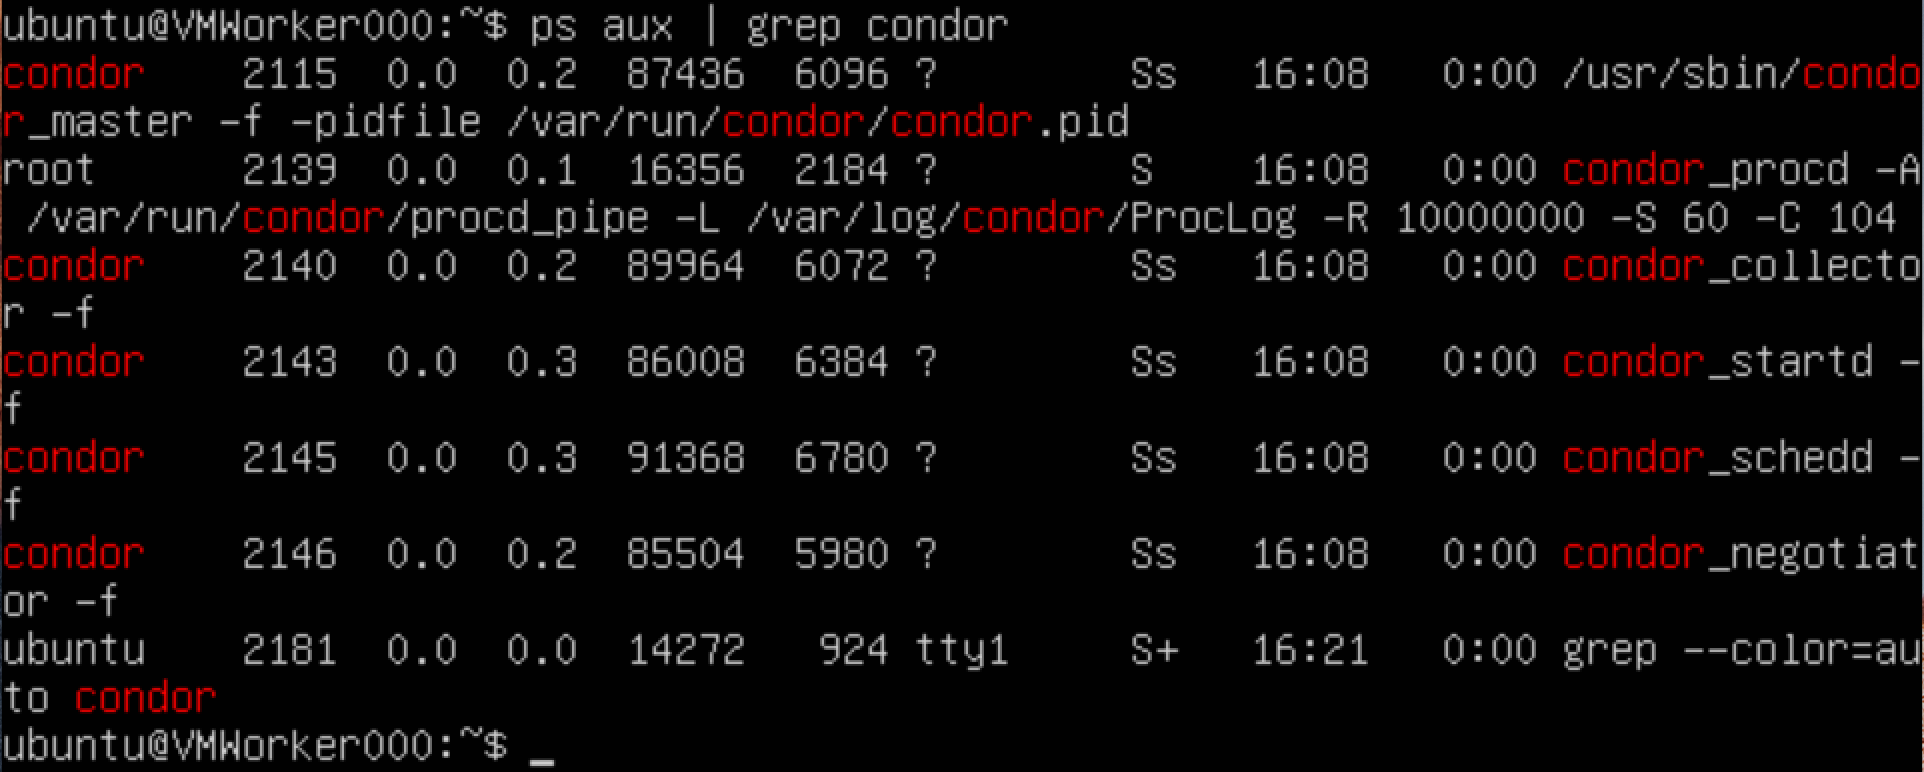
\includegraphics[width=0.8\textwidth]{Figures/running.png}
\decoRule
\caption{HTCondor activo en el sistema}
\label{fig:htcondor pre-conf}
\end{figure}
\FloatBarrier

\section{Instalación de Java}

Luego de la instalación de HTCondor, se procede con la instalación de Java en el sistema, para ello se usa un PPA con la información reciente de Java versión 8.

para ello primero instalamos la herramienta de manejo de PPA

\textbf{\textit{apt-get install software-properties-common}}

y luego agregamos el PPA correspondiente a Java.

\textbf{sudo add-apt-repository ppa:webupd8team/java}

\begin{figure}[h]
\centering
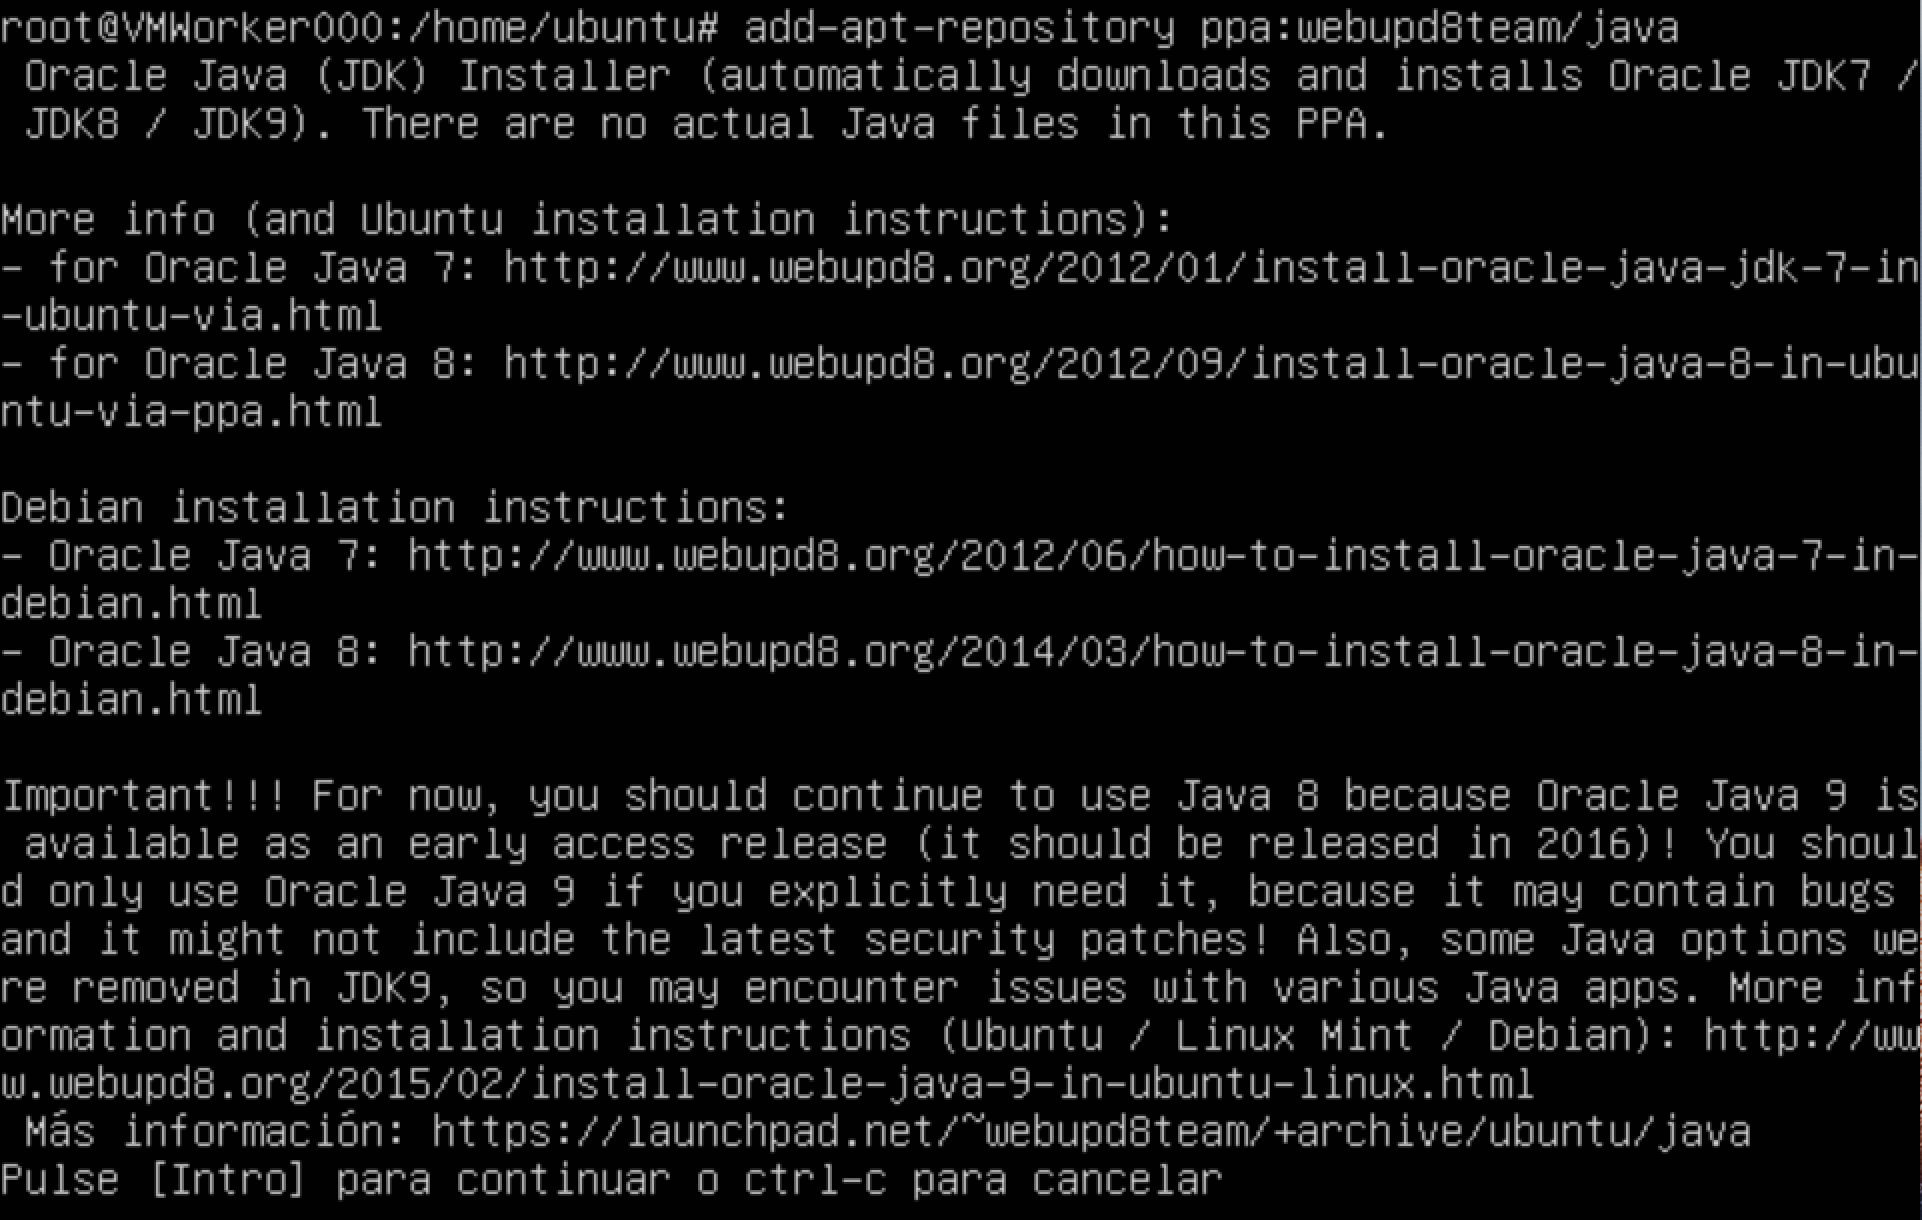
\includegraphics[width=0.8\textwidth]{Figures/ppajava.png}
\decoRule
\caption{PPA Java}
\label{fig:ppa java}
\end{figure}
\FloatBarrier

\begin{figure}[h]
\centering
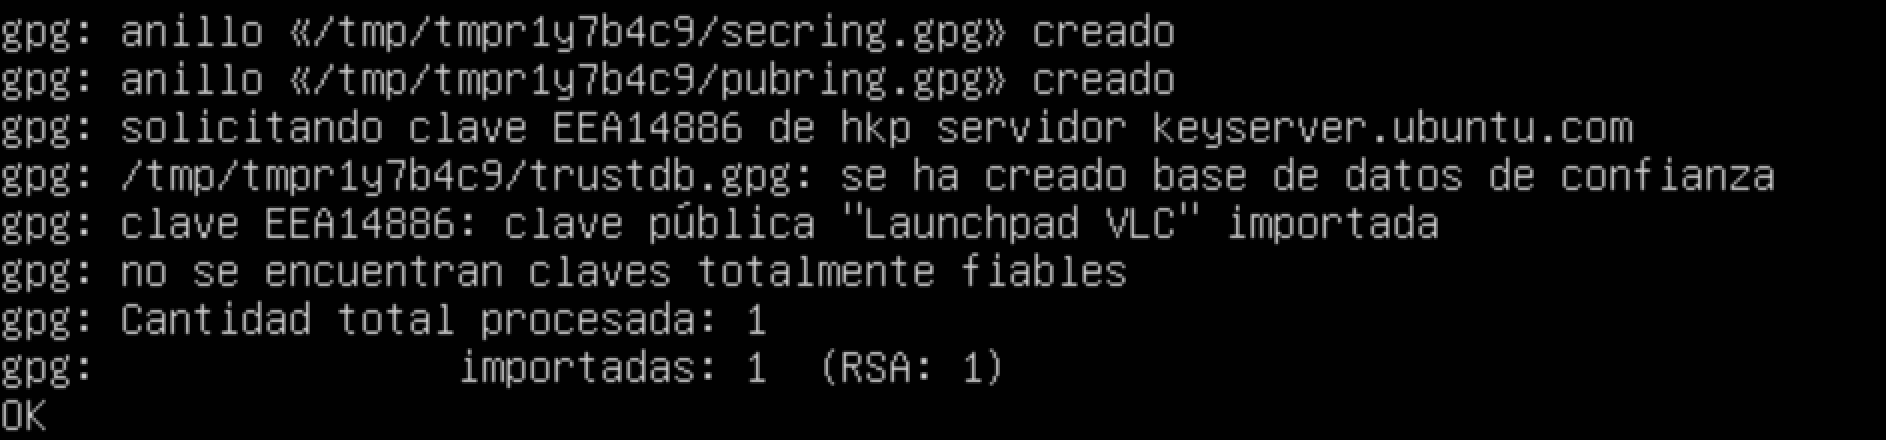
\includegraphics[width=0.8\textwidth]{Figures/ppajavaok.png}
\decoRule
\caption{PPA Java instalado}
\label{fig:ppa java aceptación}
\end{figure}
\FloatBarrier
Luego se actualiza la lista de paquetes del sistema usando el comando:

\textbf{sudo apt-get update}

Y se procede a instalar Java 8.

\textbf{sudo apt-get install oracle-java8-installer}
\begin{figure}[h]
\centering
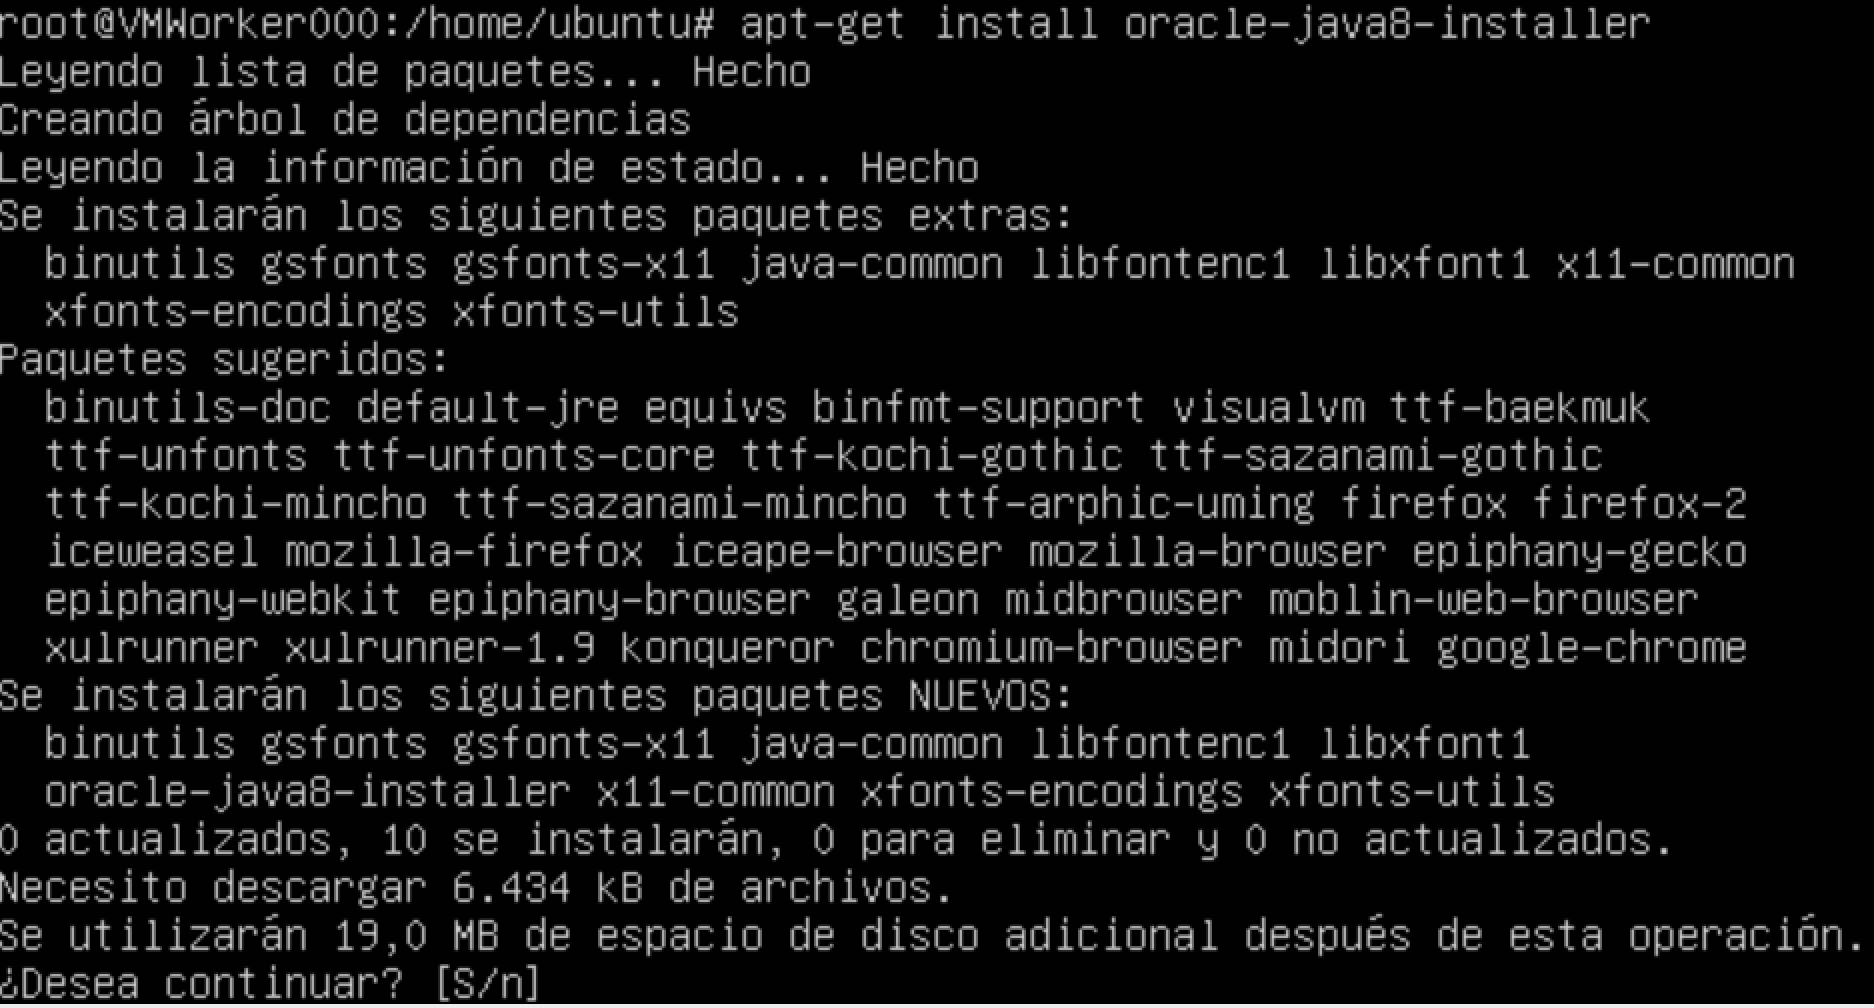
\includegraphics[width=0.8\textwidth]{Figures/javainstall.png}
\decoRule
\caption{Comando instalación de Java}
\label{fig:Java install command}
\end{figure}
\FloatBarrier

Se aceptan luego los términos y condiciones de Java 8.

\begin{figure}[h]
\centering
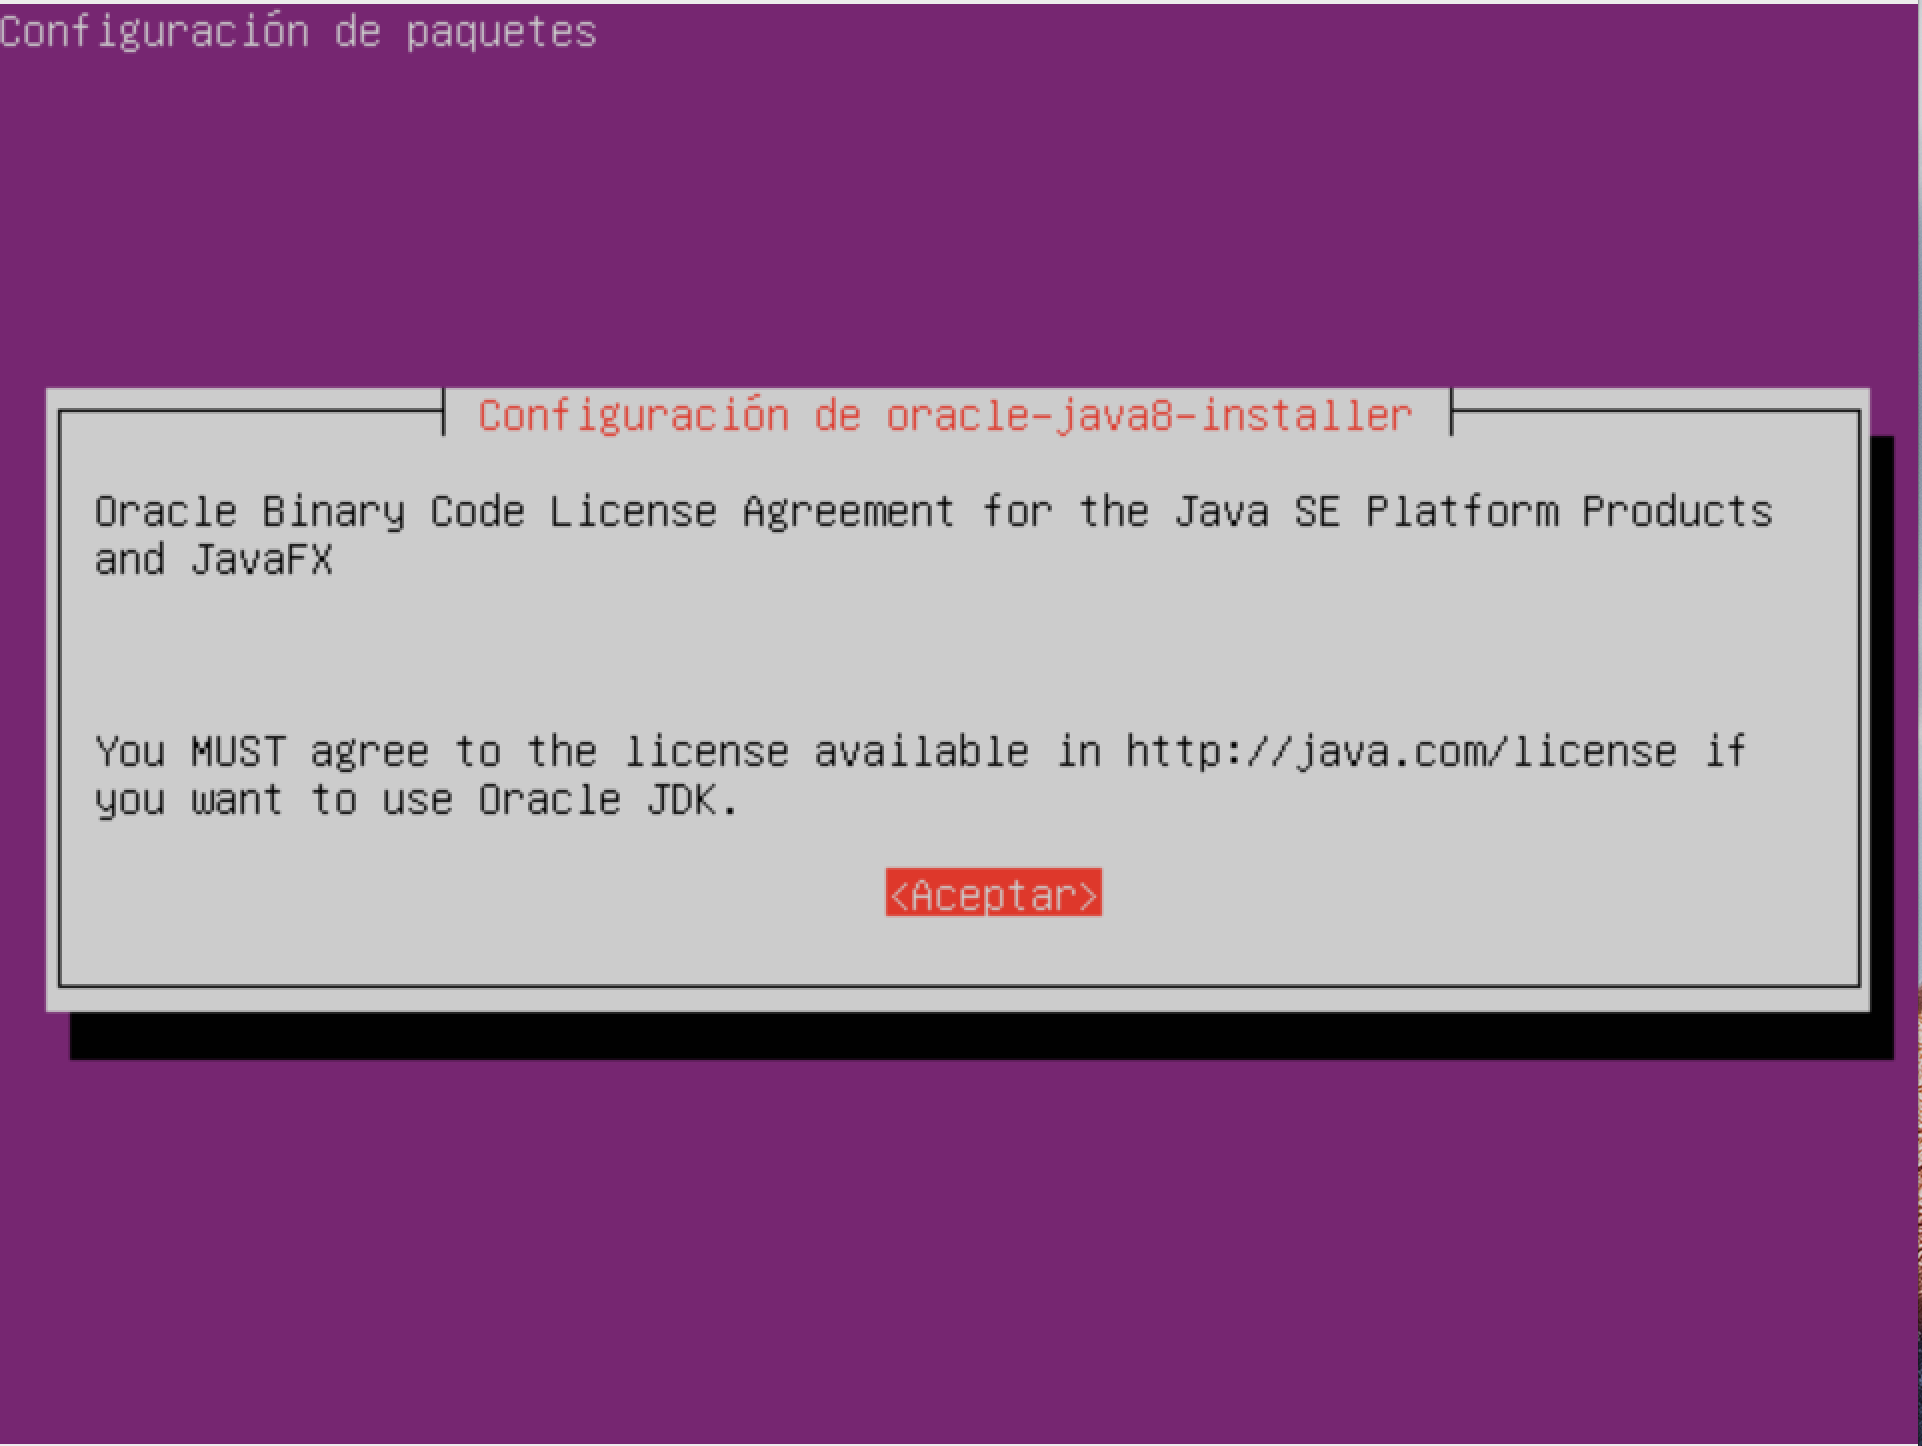
\includegraphics[width=0.8\textwidth]{Figures/javaagree.png}
\decoRule
\caption{Aceptación de instalación}
\label{fig:Java agree}
\end{figure}
\FloatBarrier

Confirmamos que java este instalado correctamente y vemos la versión del mismo con el comando:

\textbf{ java -version}

\begin{figure}[h]
\centering
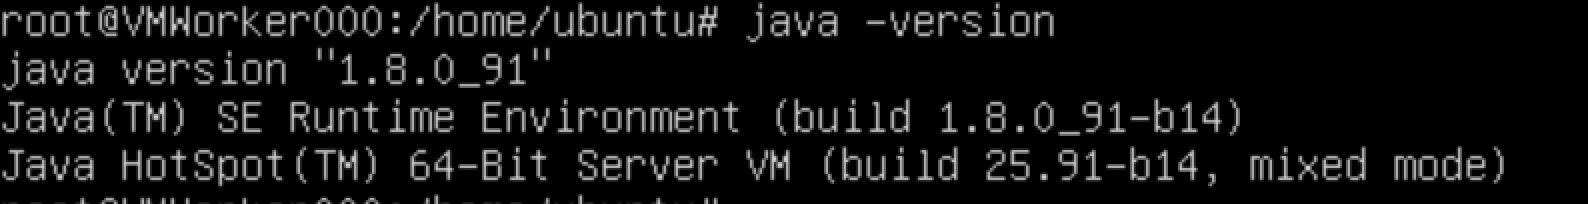
\includegraphics[width=0.8\textwidth]{Figures/javaversion.png}
\decoRule
\caption{Instalación finalizada}
\label{fig:Java version}
\end{figure}
\FloatBarrier

\section{Instalación de GCC}
Una vez instalado Java, procedemos a la instalación de las librerías y compiladores de C y C++ (\textbf{gcc}).

\textbf{apt-get install gcc}

\begin{figure}[h]
\centering
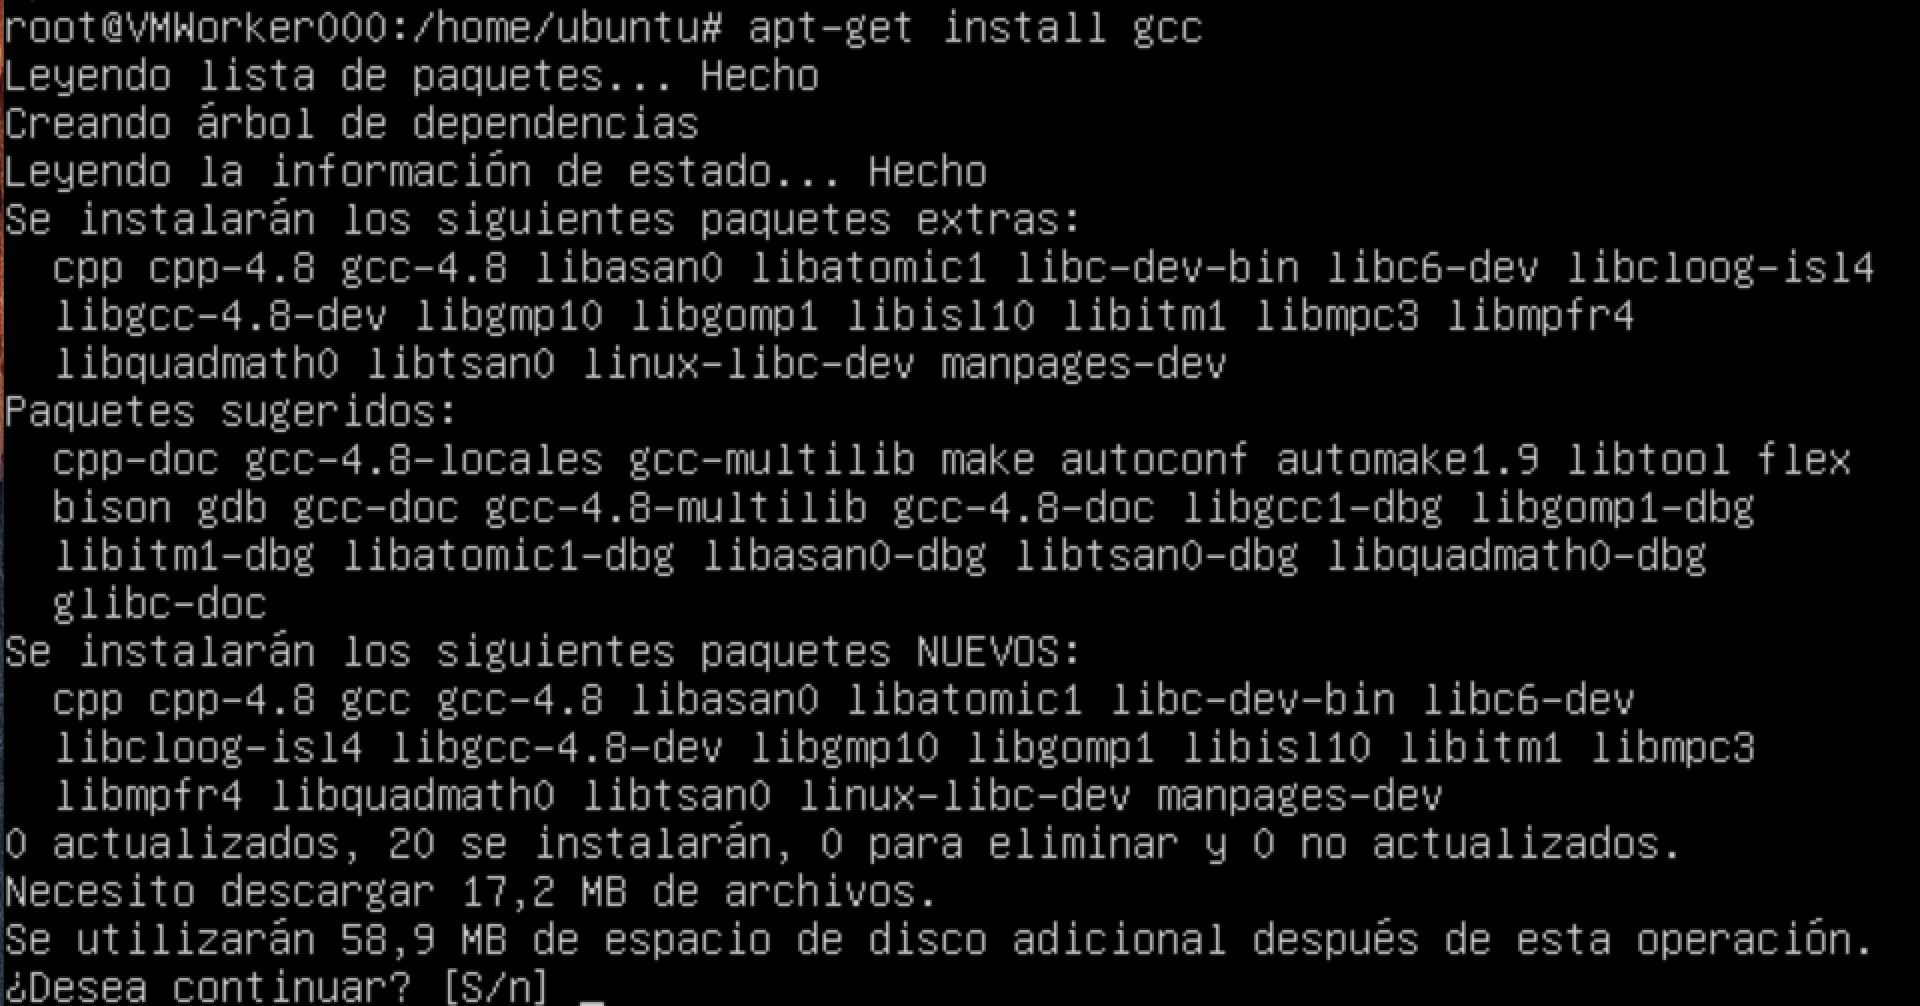
\includegraphics[width=0.8\textwidth]{Figures/gccinstall.png}
\decoRule
\caption{Instalación de gcc}
\label{fig:GCC install}
\end{figure}
\FloatBarrier
Verificamos la instalación de gcc con el comando:

\textbf{which gcc}

\begin{figure}[h]
\centering
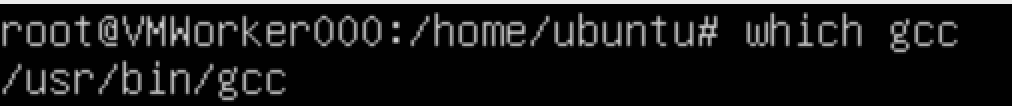
\includegraphics[width=0.8\textwidth]{Figures/gccok.png}
\decoRule
\caption{gcc instalado}
\label{fig:GCC ready}
\end{figure}
\FloatBarrier

En la carpeta del usuario, hay un ejemplo un programa en c que corre el famoso Hola mundo! ( Hola, UTB! ) que muestra el funcionamiento de las librerías de c y c++

\begin{figure}[h]
\centering
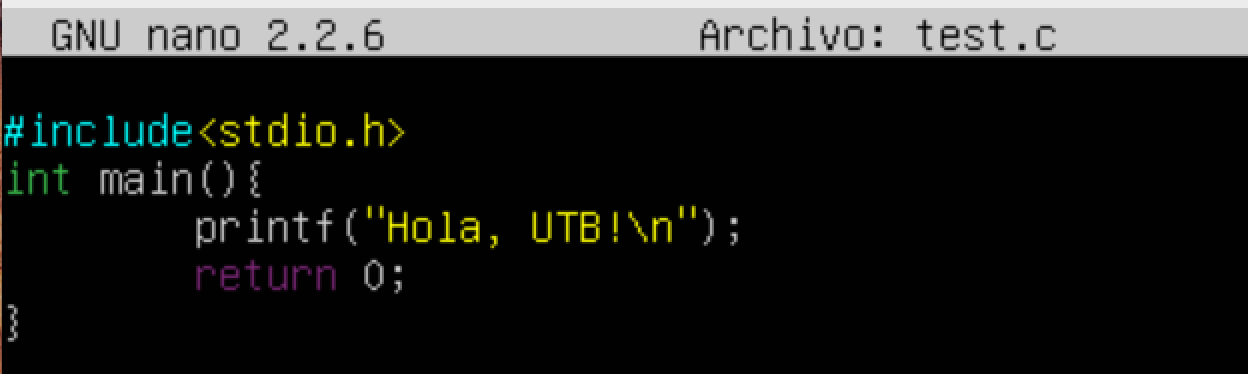
\includegraphics[width=0.8\textwidth]{Figures/pruebagcc.png}
\decoRule
\caption{Código de prueba gcc}
\label{fig:GCC program}
\end{figure}
\FloatBarrier

\begin{figure}[h]
\centering
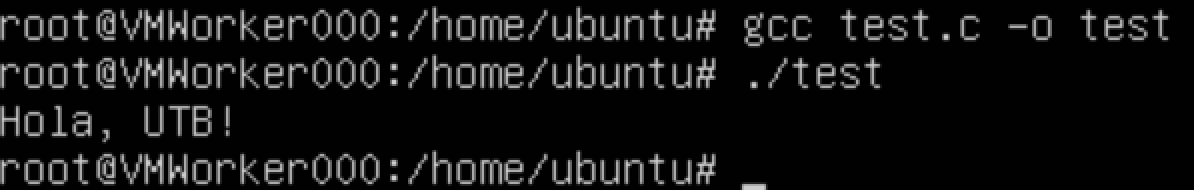
\includegraphics[width=0.8\textwidth]{Figures/testgccok.png}
\decoRule
\caption{gcc prueba de ejecución}
\label{fig:GCC test ok}
\end{figure}
\FloatBarrier

Uva vez ya configuradas las herramientas se procede a configurar HTCondor para la ejecución de tareas.
%--------------------------------------------------------